\subsection{Infraestructura y herramientas}
\subsubsection{Descripción general de la infraestructura}
La infraestructura y las herramientas son la base sobre la que se construirán
los diferentes proyectos de aprendizaje automático. Se encargan de proporcionar
un entorno de desarrollo e investigación eficiente, que permita a los miembros
del equipo centrarse en el desarrollo de modelos sin tener que preocuparse por
la configuración. Concretamente, se han desplegado dos plataformas 
que vienen a cubrir varias de las necesidades fundamentales de los proyectos
como son la gestión y exploración de datasets, la monitorización de experimentos o
el almacenamiento de modelos de inteligencia artificial. Además, se ha añadido un sistema de autenticación 
para garantizar la seguridad y privacidad de los datos.\medskip

Esta infraestructura se ha desplegado en un servidor interno de la empresa
utilizando contenedores de Docker. La elección de esta tecnología se debe a
que permite la creación de entornos aislados y portables, lo que facilita el
despliegue de las aplicaciones. Se ha utilizado Docker Compose para
sincronizar el despliegue de los diferentes servicios, lo que permite
realizar despliegues automatizados mediante las acciones de GitLab CI. La
figura \ref{fig:internal-server} muestra una vista general de la infraestructura
desplegada en el servidor interno de la empresa, donde se pueden observar
como se integran los diferentes servicios y sus respectivas conexiones. Además,
se puede observar que todos los servicios están interconectados mediante un
proxy inverso mediante Nginx, que se encarga de redirigir las peticiones en 
función de la URL. Esto permite que todos los servicios sean
accesibles desde el exterior a través de un único punto de entrada y que el
sistema de autenticación sea común para todos ellos.

\begin{figure}[ht]
    \centering
    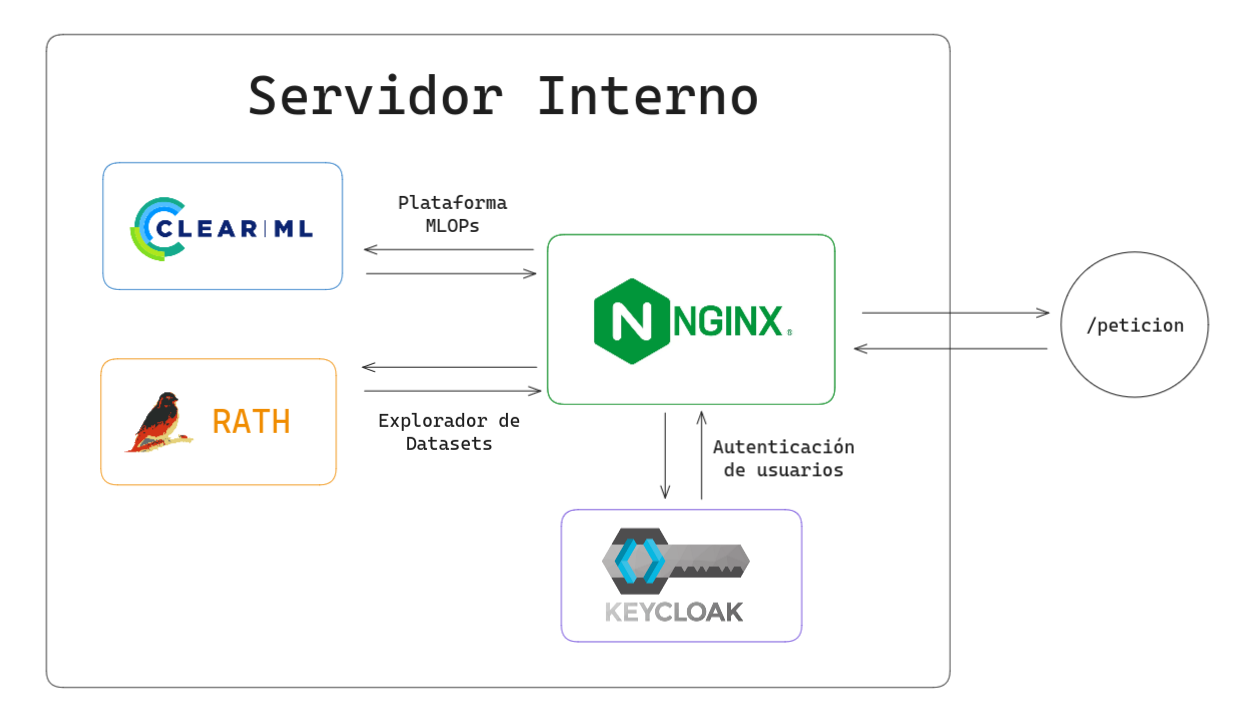
\includegraphics[width=\textwidth]{internal-server.png}
    \caption{Vista general del servidor interno.}\label{fig:internal-server}
\end{figure}

\subsubsection{Selección de plataformas}
Previo a la elección de las plataformas integradas, se realizó una evaluación
a nivel de equipo para determinar las necesidades que se debían cubrir. Se
identificaron las siguientes funcionalidades fundamentales:

\begin{itemize}
    \item \textbf{F1:} Versionado y almacenamiento de dataset.
    \item \textbf{F2:} Monitorización de experimentos.
    \item \textbf{F3:} Almacenamiento de modelos de inteligencia artificial.
    \item \textbf{F4:} Integración de métricas en datasets y visualización de resultados.
    \item \textbf{F5:} Exploración de datasets.
\end{itemize}

Una vez identificadas las necesidades, se consensuó un criterio de selección
para las plataformas integradas. Este criterio es un criterio de mínimos, es
decir, se seleccionarán las plataformas que cumplan con el criterio mínimo
establecido y que, además, ofrezcan funcionalidades adicionales que puedan
ser de utilidad para el equipo. El criterio de selección se basa en los
siguientes aspectos: 

\begin{itemize}
    \item \textbf{C1 (Facilidad de uso):} se valora muy positivamente la facilidad de uso de las
    plataformas, ya que se considera que no todo el equipo no tiene experiencia
    previa en el uso de estas herramientas.
    \item \textbf{C2 (Integración con otras herramientas):} es fundamental que las
    plataformas integradas sean compatibles con las librerías y herramientas
    que se utilizan generalmente en proyectos (TensorFlow, PyTorch, etc.).
    \item \textbf{C3 (Poca dependencia sobre la infraestructura):} se mide la dependencia
    sobre una plataforma como el numero de acciones que se deben realizar para
    migrar un proyecto estándar, es decir, un proyecto que no ha sido
    desarrollado con la plataforma en mente. Y penalizando aquellas practicas
    que sean propias de la plataforma y que no sean comunes en la industria.
\end{itemize}

Con estos criterios en mente, se tuvieron en cuenta las siguientes
plataformas a la hora de realizar la evaluación: MLflow, ClearML, Kedro, ZenML, Data Version Controller (DVC),
Rath, Apache Superset. Cada una de estas plataformas tiene diferentes enfoques y 
funcionalidades, pero todas ellas cubren una o varias de las necesidades fundamentales
identificadas, por lo que se consideraron candidatas para su integración en la
infraestructura. La infraestructura final se compondrá de una o varias de estas
plataformas en función de los criterios previamente establecidos. A continuación, se 
muestra un análisis detallado de las plataformas evaluadas y las funcionalidades que ofrecen.\medskip

\begin{itemize}
    \item \textbf{MLflow:} MLflow \cite{WhatMLflow} es una plataforma MLOPs de código abierto para la gestión del ciclo de vida de
    los modelos. Ofrece una interfaz de usuario para el seguimiento de experimentos, la gestión de modelos 
    y la implementación de modelos en diferentes entornos. MLflow es compatible con la mayor parte de librerías de aprendizaje 
    automático, como TensorFlow o PyTorch. Uno de los puntos fuertes de MLflow es su gran comunidad, ya que es
    una de las plataformas más utilizadas en la industria. Sin embargo, no ofrece funcionalidades relacionadas con
    la gestión, evaluación o versionado de datasets ni con la exploración de los mismos. La dependencia sobre la
    plataforma varía en función de la tarea que se quiera realizar, pero en general, es una plataforma que no
    ata al usuario a su ella. La documentación se queda corta en cuestión de claridad y ejemplos, lo que puede
    dificultar la adopción de la plataforma por parte de los miembros del equipo.
    \item \textbf{ClearML:}Similar a MLflow, ClearML \cite{WhatClearML} es una plataforma MLOps de código abierto que ofrece funcionalidades para la 
    gestión de experimentos, pero con la ventaja de incluir herramientas para la gestión, evaluación y 
    versionado de datasets. La dependencia sobre la plataforma es mínima, ya que con pocos cambios se pueden 
    lanzar experimentos y adicionalmente permite el lanzamiento de pipelines, gestión de alertas, orquestación de modelos 
    y generación de puntos de acceso para modelos ya desplegados. Aunque es compatible con muchas bibliotecas populares su comunidad 
    es más limitada, lo que puede dificultar a la hora de encontrar soluciones a ciertas problemáticas.
    La documentación es clara y ofrece ejemplos en formato tanto en formato de blog como de video facilitando la 
    comprensión. Sin embargo, carece de un sólido sistema de autenticación por defecto, lo que requiere una
    implementación adicional para proteger correctamente la aplicación web.
    \item \textbf{Data Version Controller (DVC):} DVC \cite{dvc} es una herramienta de código abierto que
    están diseñadas para manejar grandes volúmenes de datos, modelos y experimentos. DVC
    se centra en el versionado y almacenamiento de datasets, mientras que DVC Studio se centra en la
    monitorización de experimentos, visualización de resultados y almacenamiento de modelos, pero a diferencia
    de DVC esta es una herramienta de pago. DVC proporciona integraciones con un número considerable de librerías de 
    aprendizaje automático. La documentación está bien estructurada aunque no es tan clara como la de ClearML, pero cuenta con una
    comunidad bastante activa. En cuanto a los aspectos negativos de DVC, la principal desventaja es que
    la curva de aprendizaje es bastante pronunciada, lo que dificulta su adopción. Otro punto en contra
    es la gran dependencia que tienen los proyectos que usan DVC, ya que se necesita de varios archivos
    de configuración, integraciones manuales dentro del código y un dominio completo de los comandos de la
    herramienta para poder trabajar con ella. Además, funcionalidades clave como la visualización son funcionalidades
    de pago en DVC Studio, lo que limita su uso en la capa gratuita.
    \item \textbf{ZenML:} ZenMl es una plataforma de código abierto encargado de la orquestación de pipelines en
    proyectos de aprendizaje automático. Ofrece una experiencia de desarrollo cómoda y modular, que facilita
    la reutilización de código. Además, cuenta con integraciones para las platformas de almacenamiento
    mas populares, como AWS y Google Cloud. A diferencia de ClearMl y MLflow, este no está enfocado en la
    gestión de experimentos ya que no es una plataforma MLOps, aunque si que ofrece conexiones con esta última
    para poder redireccionar nuestros experimentos. La documentación es clara y podemos encontrar diversos repositorios 
    con ejemplos de uso o integración con otras herramientas. El problema de esta radica principalmente
    en el hecho de que al no ser una plataforma MLOps, no ofrece funcionalidades relacionadas con la gestión
    o versionado de datasets, lo que es un punto negativo para nuestro caso de uso. Otro de los problemas
    es que las plataformas que integra no comparten las mismas credenciales dentro de su capa
    gratuita, lo que dificulta en gran medida su uso. 
    \item \textbf{Kedro:} Al igual que ZenML, Kedro es una plataforma de código abierto que se centra en la
    orquestación de pipelines en proyectos de aprendizaje automático. Otra diferencia respectiva a ZenML es
    que Kedro no ofrece compatibilidad con ningún tipo de plataforma MLOPs, en cambio, trae su propia herramienta
    e implementación propia de la mayoría de funcionalidades de orquestación. Su herramienta de consola es configurable 
    y compatible con Cookiecutter, lo que facilita la creación de plantillas personalizadas. Por otro lado, al
    ser muy similar a ZenML, Kedro tampoco ofrece funcionalidades relacionadas con la gestión de experimentos,
    lo que es un punto negativo para nuestro caso de uso. 
    \item \textbf{Rath:} herramienta de exploración de datasets que permite una exploración semi-automática
    de datasets. Muy fácil de utilizar, ya que cuenta con un modo copilot que te sugiere di\-fe\-ren\-tes gráficos
    y estadísticas en función de los datos que estés explorando. Además, no requiere de ninguna configuración
    previa, ya que se puede utilizar directamente desde el navegador.
    \item \textbf{Apache Superset:} Apache Superset es una plataforma de visualización de datos de código abierto 
    que ofrece una amplia gama de características para explorar y visualizar datos de manera interactiva. Con una 
    interfaz intuitiva y basada en web, Superset permite a los usuarios crear paneles de control, gráficos y tablas 
    dinámicas con facilidad. Además, ofrece integraciones con diversas fuentes de datos y admite la creación de 
    paneles de control en tiempo real. Una de las fortalezas de Apache Superset es su comunidad activa y en constante 
    crecimiento, lo que garantiza un soporte sólido y una mejora continua de la plataforma. Sin embargo, la integración
    con el resto de herramientas es limitada, ya que el propio Superset requiere de un formato de datos concreto para
    poder subir los datos a la plataforma, lo que puede dificultar su integración y generar duplicidad en cuanto a los
    datos almacenados, ya que se necesitaría una copia de los datos en el formato que requiere Superset. Nuestro objetivo
    es que esta herramienta agilice el proceso de exploración de datos, por lo que no es una opción viable por el momento.
    \item \textbf{Grafana:} Grafana es una plataforma de análisis y visualización de métricas de código abierto que 
    se ha convertido en una opción popular para monitorear sistemas y aplicaciones. Con una amplia gama de complementos 
    y paneles personalizables, Grafana permite a los usuarios crear cuadros de mando y gráficos altamente personalizados 
    para visualizar datos de diferentes fuentes. Además, ofrece características avanzadas como alertas, anotaciones y 
    exploración de datos en tiempo real. Grafana es altamente modular y extensible, lo que facilita su integración con 
    diversas tecnologías y sistemas de monitorización. El problema de Grafana es el mismo que el de Superset, ya que requiere
    de un formato de datos concreto para poder subir los datos a la plataforma, lo que puede dificultar su integración y
    generar duplicidad en cuanto a los datos almacenados. Además, de su curva de aprendizaje, que es bastante pronunciada.
\end{itemize}

\begin{table}[ht]
    \centering 
    \begin{tabular}{lccccccccc}  
        
        \toprule
        \multirow{2}{*}{\parbox[c]{.2\linewidth}{\centering Tecnología}} & 
        \multicolumn{5}{c}{\textbf{Funcionalidades}} && 
        \multicolumn{3}{c}{\textbf{Criterios}} \\ 
        
        \cmidrule{2-6} \cmidrule{8-10}
        & {\centering F1} & {F2} & {F3}& {F4} & {F5} && {C1} & {C2} & {C3}\\
        
        \midrule
        MLflow           & --     & \check & \check & --     & --     && \check & \check & \check \\
        ClearML          & \check & \check & \check & \check & --     && \check & \check & \check \\
        DVC              & \check & \check & \check & \check & --     && --     & \check & --     \\ 
        ZenML            & --     & \check & \check & --     & --     && \check & \check & \check \\  
        Kedro            & --     & --     & \check & \check & --     && \check & \check & \check \\ 
        Rath             & --     & --     & --     & --     & \check && \check & --     & \check \\ 
        Apache Superset  & \check & --     & --     & \check & --     && --     & --     & \check \\ 
        Grafana          & \check & --     & --     & \check & --     && --     & --     & \check \\ 
        \bottomrule
        
    \end{tabular}
    \caption{Tabla comparativa de las plataformas evaluadas}
    \label{tab:comparative-table} 
\end{table}

Para finalizar con la evaluación, se puede observar en la tabla \ref*{tab:comparative-table} 
una comparativa que muestra
las funcionalidades y criterios que cumple cada una de ellas de forma resumida.
De acuerdo con la evaluación realizada, se ha decidido integrar ClearML y Rath
en la infraestructura como las plataformas finales. ClearML cubre la mayoría de
las necesidades fundamentales identificadas, ya que ofrece soluciones para la
mayoría de casos de uso, mientras que Rath complementa con la exploración de
datasets de forma sencilla e intuitiva.  

\subsubsection{Seguridad y priviacidad}
La seguridad y la privacidad de los datos son aspectos fundamentales dentro
de un entorno de trabajo empresarial, donde la confidencialidad de los datos
es una prioridad para la empresa. Por ello, ya que ClearML y Rath no cuentan
con un sistema de autenticación robusto, se ha decidido implementar un sistema
de autenticación utilizando Keycloak, que es una solución de código abierto
para la gestión de acceso. Keycloak permite a los usuarios autenticarse con
cuentas de usuario gestionadas por la empresa, lo que garantiza que solo los
usuarios autorizados puedan acceder a los datos. Además, ofrece integraciones
con diferentes proveedores de identidad, lo que facilita la gestión de
usuarios y la integración con otras herramientas.\medskip

Debido a que tanto ClearML como Rath no tienen integraciones directas con
Keycloak, se ha decidido utilizar Nginx como proxy inverso para redirigir
las peticiones a los servicios de ClearML y Rath. De esta forma, se puede
utilizar Keycloak para autenticar a los usuarios y garantizar la seguridad
y la privacidad de los datos. La figura \ref{fig:internal-server} muestra
cómo se ha integrado Keycloak en la infraestructura, así como las conexiones
entre los diferentes servicios y el proxy inverso. En el momento actual, se
ha implementado un sistema de autenticación básico, pero se espera que en el
futuro este sistema se sincronice con el sistema de autenticación de Tecnalia
para una mayor comodidad por parte de los usuarios.

\subsubsection{Despligue Automatizado}
Para la automatización del despliegue de la infraestructura se ha utilizado
GitLab CI, una herramienta de integración y despliegue continuo que
permite automatizar el proceso de despliegue de aplicaciones. GitLab CI
permite definir un conjunto de pasos que se ejecutarán cada vez que se
realice un cambio en el repositorio, lo que facilita el despliegue de
aplicaciones y la gestión de la infraestructura.\medskip

Para poder utilizar GitLab CI, es necesario primero definir un runner, que
es un agente que se encarga de ejecutar los pasos definidos en el archivo
de configuración. En este caso, el runner se ha desplegado en el servidor
lo que permite ejecutar los diferentes flujos en el mismo entorno. Además,
otro aspecto a tener en cuenta es que por seguridad, se ha configurado el
sistema con variables de entorno que enmascaran las credenciales de acceso
a los diferentes servicios, lo que garantiza que las credenciales no se
almacenen en el repositorio. En cuanto a las pipelines, se han definido 
tres diferentes flujos para automatizar cada uno de los procesos de 
instalación y actualización:

\begin{itemize}
    \item \textbf{Instalación de autenticación:} Se encarga de instalar Keycloak
    en el servidor junto con la base de datos. Este flujo se ejecutará si no
    se ha instalado Keycloak previamente.
    \item \textbf{Instalación de infraestructura:} Se encarga de instalar ClearML y Rath
    en el servidor. Además, también se encarga de configurar el proxy inverso
    para redirigir las peticiones a los servicios de ClearML y Rath. Este flujo
    se ejecutará si no se ha instalado ClearML previamente.
    \item \textbf{Despliegue de infraestructura:} Se encarga de actualizar el
    servidor a los nuevos cambios realizados en el repositorio. Este flujo se
    lanza cada vez que detecta un cambio en el repositorio, pero requiere de
    una aprobación manual para ejecutarse.
\end{itemize}

La idea de estos flujos es que se puedan ejecutar de forma independiente
y que en caso de que se necesite realizar un cambio en la infraestructura,
se pueda lanzar el flujo en otro servidor para instalar la infraestructura
de forma automática. Además, facilita el trabajo en local, ya que una vez
automatizado el despliegue, los cambios en local se pueden probar lanzar
directamente en el servidor.

\subsubsection{Problemas durante el Despliegue}
A continuación se detallan la lista de problemas que se han encontrado durante
el despliegue de la infraestructura y las soluciones que se han aplicado para
resolverlos. Estos soluciones se detallan con el fin de que puedan ser de utilidad
para futuros despliegues o como registro para mejoras futuras.

\begin{itemize}
    \item \textbf{Clearml no es compatible con servidores no IPv6.} Por defecto,
    ClearML utiliza direcciones IPv4 e IPv6 para comunicarse con el servidor. Sin
    embargo, en el servidor interno de la empresa no está habilitado el soporte
    para direcciones IPv6, lo que provoca que ClearML no pueda comunicarse con el
    servidor. Internamente, ClearML utiliza una configuración de Nginx para esta
    comunicación, pero no es posible modificarla directamente ya que el contenedor de
    Docker lanza un script en bash que sobrescribe la configuración de Nginx y luego lanza
    el servidor. La solución a este problema es sobrescribe una variable interna llamada
    \textit{DISABLE\_NGINX\_IPV6} dentro del contenedor de Webserver de ClearML. Este
    error es común pero no está documentado en la documentación oficial, la solución
    es una propuesta personal que ha sido descubierta mediante la lectura del código.
    \item \textbf{ClearML no renderiza correctamente en el navegador.} Otro de los problemas
    que encontramos al desplegar ClearMl es que el servidor interno de la empresa no
    era capaz de servir archivos estáticos de un tamaño superior a 3.5MB. Esto provocaba
    que la interfaz de usuario de ClearML no se renderizara correctamente los gráficos,
    ya que internamente utiliza plotly para la visualización de los mismos. La solución
    a este problema fue recompilar la libreria de plotly por nuestra cuenta incluyendo
    solamente los gráficos que necesitamos, de esta forma reducimos el tamaño de los
    archivos estáticos y conseguimos que la interfaz de usuario se renderizara correctamente.
\end{itemize}